\documentclass{exam}
%\documentclass[answers]{exam}
\hbadness=99999
\usepackage[total={6.5in,9in}]{geometry}

\usepackage{enumerate}
\usepackage{amsmath}
\usepackage[table]{xcolor}
\usepackage{graphicx}
\usepackage{tikz}
\usepackage{pgf-umlcd}
\usepackage{multicol}

% for UML colors
\renewcommand{\umlfillcolor}{orange!10}
\renewcommand{\umldrawcolor}{black}

% for syntax highlighting
\usepackage{minted}
\usemintedstyle[cpp]{xcode}

% for overlay of output
\usepackage[overlay,showboxes]{textpos}

\pagestyle{plain}

\setlength\columnsep{50pt}
\newcommand{\key}{\hfill
      \raisebox{-.3\height}{\includegraphics[width=0.6in]{figures/key.png}}}

\begin{document}
  \thispagestyle{empty}
  \setlength{\parindent}{0pt}

  \begin{center}
    \Large Activity \#4: UML and Class Design \\[5pt]
    \large Recorder's Report\\[20pt]
    \normalsize
    \begin{tabular}{lrp{0.1in}lr}
      Manager:  & \fillin[][2.0in] & & Presenter: & \fillin[][2.0in]\\[15pt]
      Recorder: & \fillin[][2.0in] & & Driver:    & \fillin[][2.0in]\\[15pt]
      Date:     & \fillin[][2.0in] & & Score:     & Satisfactory \hspace{10pt} /
      \hspace{10pt} Not Satisfactory
    \end{tabular}
  \end{center}
  \par\vskip 15pt
  
  Record your group's answers to the key questions (marked with
  \raisebox{-.3\height}{\includegraphics[width=0.5in]{figures/key.png}})
  below.
  \begin{enumerate}[(a)]
    \itemsep 1.75in
    \item Model 1, Question \#4
    \item Model 2, Question \#8
    \item Model 2, Question \#11
  \end{enumerate}

  \clearpage\pagenumbering{arabic} 
  
  \begin{center}
    \Large Activity \#4: UML And Class Design \\[5pt]
    \large Activity Guide\\[20pt]
  \end{center}

  \begin{center}
    \fbox{
      \begin{minipage}{5.5in}
        {\bf Learning Objectives:} Students will be able to:
        \begin{itemize}
          \item Content:\\[-20pt]
            \begin{itemize}           
              \itemsep 0pt
              \item Explain class diagrams in UML
              \item Implement a class based on a UML diagram
            \end{itemize}
          \item Process\\[-20pt]
            \begin{itemize}
              \itemsep 0pt
              \item Write method signatures exactly as shown in a UML diagram
              \item Design a new class as a UML diagram based on a general description\\[-5pt]
            \end{itemize}
        \end{itemize}
      \end{minipage}
      }
  \end{center}
  \par\vskip 10pt
  
  
  {\bf\large Model 1: The Die Class}\\[-10pt]
  \begin{center}
    \footnotesize
    \renewcommand{\arraystretch}{1.2}
    \begin{tabular}{p{1.5in}p{2.5in}p{1in}}
      \begin{minipage}{1.5in}
        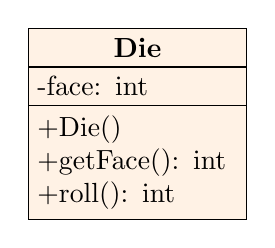
\begin{tikzpicture}
          \begin{class}[text width=1in]{Die}{0,0}
            \attribute{-face: int}
            \operation{+Die()}
            \operation{+getFace(): int}
            \operation{+roll(): int}
          \end{class}
        \end{tikzpicture}
      \end{minipage}
      & 
      \begin{minipage}{2.5in}
        \begin{minted}[
          frame=lines,
          framesep=2mm,
          bgcolor=gray!15,
          baselinestretch=1.2,
          linenos,
          firstnumber=6
        ]{cpp}
class Die {
  public:
    Die() { this->face = 1; }
    int getFace() const {
      return this->face;
    }
    int roll() {
      this->face = rand() % 6 + 1;
      return this->face;
    }
  private:
    int face;
};
        \end{minted}   
      \end{minipage}
      &
      \begin{minipage}{1in}
        \centering
        \includegraphics[width=1in]{figures/dice.png}
      \end{minipage}
    \end{tabular}
  \end{center}
  \par\vskip 5pt
  
  {\it\large Refer to Model 1 above as your group develops consensus answers
    to the questions below.}
    \par\vskip 10pt
    
  \begin{enumerate}
    \itemsep 20pt
    
    \item In the {\it Unified Modeling Language} (UML), a class diagram
      (on the left in our model) provides a way of graphically 
      illustrating a class's design, independent of programming language. 
      \par\vskip 10pt
      
      \begin{enumerate}[(a)]
        \item What are the attributes of {\tt Die} and what are its
          methods?
          \begin{solution}[1in]
            The only attribute is {\tt face} and the methods are {\tt
            Die}, {\tt roll}, and {\tt getFace}.
          \end{solution}
        \item How are attributes and methods distinguished in the
          class diagram?
          \begin{solution}[1in]
            The attributes are in the first block of the diagram below
            the title.  The methods are in the second block after the
            attributes.
          \end{solution}
      \end{enumerate}

\newpage

      \item Notice that several special symbols are used in the class
        diagram.  Compare the diagram with the given C++ implementation
        of the class to help you answer the following questions.
        \par\vskip 10pt
        
        \begin{enumerate}
          \item In the class diagram, what do the ``{\tt -}'' and
            ``{\tt +}'' symbols represent?
            \begin{solution}[0.75in]
              The plus means that the attribute or method is public.
              The minus means it is private. 
            \end{solution}
          \item What does the ``{\tt :}'' represent?
            \begin{solution}[0.75in]
              The colon refers to the data type.
            \end{solution}
        \end{enumerate}

    \item The file {\tt activity04a.cpp} contains the class from this
      model along with an example {\tt main} program that utilizes it.
      \par\vskip 10pt
      
      \begin{enumerate}
        \item What would you change to make this a 5-sided die?        
          \begin{solution}[0.75in]
            You would change the code on line 13 to read
            \begin{center}
              \mintinline{cpp}|this->face = rand() % 5 + 1;|
            \end{center}
          \end{solution}
        \item How would you change the class diagram to reflect this
          change in the code?
          \begin{solution}[0.75in]
            You would not change it at all.
          \end{solution}
      \end{enumerate}
      \vskip -40pt\null

    \item Suppose you wanted to generalize this class so that it could
      represent a die with any\key\\[-2.5mm] number of sides, set by the constructor.  
      \par\vskip 10pt
      
      \begin{enumerate}[(a)]
        \item What new attribute(s) and/or method(s) would you need to add?
          \begin{solution}[0.75in]
            We would need to add an attribute for {\tt numFaces}.
          \end{solution}
        \item What methods would you need to alter?
          \begin{solution}[0.75in]
            We would need to alter the constructor to set the number
            of faces, and we would need to change the {\tt roll} method
            to use the number of faces in computing a random value.
          \end{solution}
        \item What would the class diagram look like after these changes?
          \begin{solution}[0.75in]
            \begin{tabular}{|l|}
              \hline
              \rowcolor{orange!20}\multicolumn{1}{|c|}{\bf Die}\\
              \hline
              \rowcolor{white} \tt -face: int\\
              \tt -numFaces: int\\
              \hline
              \tt +Die(numFaces: int)\\
              \tt +getFace(): int\\
              \tt +roll(): int\\
              \hline
            \end{tabular}
          \end{solution}
      \end{enumerate}
      
\newpage

  {\bf\large Model 2: A Circle Class}\\[-10pt]
  \begin{center}
    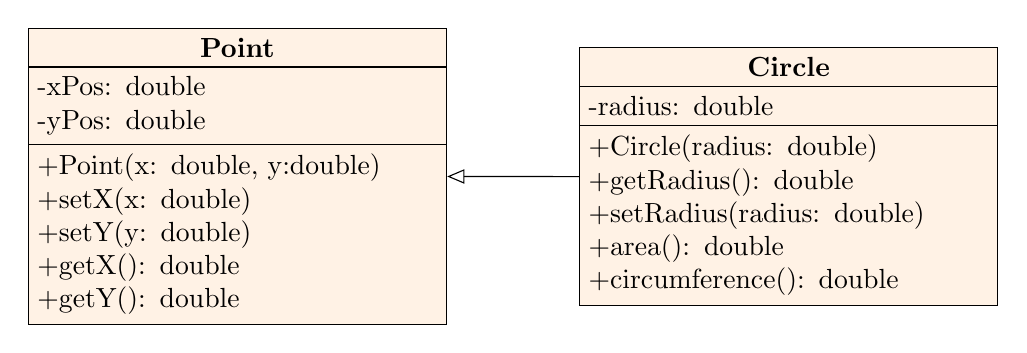
\begin{tikzpicture}
      \begin{class}[text width=2in]{Point}{0,0}
        \attribute{-xPos: double}
        \attribute{-yPos: double}
        \operation{+Point(x: double, y:double)}
        \operation{+setX(x: double)}
        \operation{+setY(y: double)}
        \operation{+getX(): double}
        \operation{+getY(): double}
      \end{class}
      \begin{class}[text width=2in]{Circle}{7,-0.25}
        \inherit{Point}
        \attribute{-radius: double}
        \operation{+Circle(radius: double)}
        \operation{+getRadius(): double}
        \operation{+setRadius(radius: double)}
        \operation{+area(): double}
        \operation{+circumference(): double}
      \end{class}
    \end{tikzpicture}
  \end{center}
  
  {\it\large Refer to Model 2 above as your group develops consensus answers
    to the questions below.}
  \par\vskip 10pt
    
  \item What are the attributes and methods of {\tt Circle}, and what
    is their visibility?
    \begin{solution}[0.75in]
      The attributes and methods are:
      \begin{itemize}
        \item Attribute {\tt radius} is private
        \item Methods {\tt Circle}, {\tt area}, {\tt circumference},
          {\tt getRadius}, and {\tt setRadius} are all public.
      \end{itemize}
    \end{solution}
    
  \item Based on this model and the previous one, what parts of a
    class are typically private, and what parts are typically public?
    \begin{solution}[0.75in]
      The attributes are typically private and the methods are
      typically public.
    \end{solution}
          
  \item What does the arrow pointing from the {\tt Circle} class
    diagram to the {\tt Point} class diagram represent?
    \begin{solution}[0.75in]
      It represents the ``is-a'' relationship whereby {\tt Circle} inherits
      the properties of {\tt Point}.
    \end{solution}
    
  \item The file {\tt activity04b.cpp} contains an implementation of
    the {\tt Point} class.  Write  an\key\\[-2.5mm] implementation of the {\tt
    Circle} class that matches this diagram.
    \begin{solution}{1.5in}
      \begin{minipage}{3in}
        \begin{minted}[
          frame=lines,
          framesep=2mm,
          bgcolor=gray!15,
          baselinestretch=1.2,
          linenos,
        ]{cpp}
                
        \end{minted}
      \end{minipage}
    \end{solution}

\newpage
  
  {\bf\large Model 1: A Credit Card}\\[-10pt]
  \begin{center}
    \includegraphics[height=1in]{figures/credit-card.png}   
  \end{center}
  
  {\it\large Refer to Model 3 above as your group develops consensus answers
    to the questions below.}    
  \par\vskip 10pt
  
  \item List two or more attributes that would be necessary for a
    class to model a {\tt CreditCard}.  Indicate what data types would
    be most appropriate.
    
    \begin{solution}[0.75in]
      Most likely we would want:
      \begin{itemize}
        \begin{multicols}{2}
          \item \verb|number:long|
          \item \verb|expire:Date|
          \item \verb|name:String|
          \item \verb|CCV:int|
        \end{multicols}
      \end{itemize}
    \end{solution}
    
  \item When constructing or updating a {\tt CreditCard} objects, what
    values would you need to check?  What are the valid ranges of each
    attribute?
    \begin{solution}[0.75in]
      \begin{itemize}
        \item The number should have 16 digits
        \item Dates need to have valid months and years
        \item Names should be at most 22 letters long and not contain
          non-alphabet characters.
        \item CCV codes should be 3 or 4 digits long
      \end{itemize}
    \end{solution}
    \vskip -20pt\null
    
  \item Draw a UML class diagram for your implementation of the 
    {\tt CreditCard} class.\key\\[-2.5mm]
    \begin{solution}[1.25in]
    \end{solution}
    
  \item Many banks offer {\tt CashBack} credit cards which accumulate
    a certain number of points for every dollar spent.  Other banks
    offer {\tt TravelRewards} cards which accumulate miles on a
    particular airline for every dollar spent.  Construct a UML diagram 
    with appropriate attributes and methods showing classes for these
    two types of cards and their relationship to the original {\tt
    CreditCard} class you defined above.
    \begin{solution}[1.25in]
    \end{solution}
  
  \end{enumerate}
  
  
    
\end{document}
